\documentclass{article}

% if you need to pass options to natbib, use, e.g.:
%     \PassOptionsToPackage{numbers, compress}{natbib}
% before loading neurips_2026

% The authors should use one of these tracks.
% Before accepting by the NeurIPS conference, select one of the options below.
% 0. "default" for submission
\usepackage{neurips_2026}
% the "default" option is equal to the "main" option, which is used for the Main Track with double-blind reviewing.
% 1. "main" option is used for the Main Track
%  \usepackage[main]{neurips_2026}
% 2. "position" option is used for the Position Paper Track
%  \usepackage[position]{neurips_2026}
% 3. "eandd" option is used for the Evaluations & Datasets Track
 % \usepackage[eandd]{neurips_2026}
 % if you want to opt-in for a de-anomymized submission (not recommended, but OK):
 %\usepackage[eandd, nonanonymous]{neurips_2026}
% 4. "creativeai" option is used for the Creative AI Track
%  \usepackage[creativeai]{neurips_2026}
% 5. "sglblindworkshop" option is used for the Workshop with single-blind reviewing
 % \usepackage[sglblindworkshop]{neurips_2026}
% 6. "dblblindworkshop" option is used for the Workshop with double-blind reviewing
%  \usepackage[dblblindworkshop]{neurips_2026}

% After being accepted, the authors should add "final" behind the track to compile a camera-ready version.
% 1. Main Track
 % \usepackage[main, final]{neurips_2026}
% 2. Position Paper Track
%  \usepackage[position, final]{neurips_2026}
% 3. Evaluations & Datasets Track
 % \usepackage[eandd, final]{neurips_2026}
% 4. Creative AI Track
%  \usepackage[creativeai, final]{neurips_2026}
% 5. Workshop with single-blind reviewing
%  \usepackage[sglblindworkshop, final]{neurips_2026}
% 6. Workshop with double-blind reviewing
%  \usepackage[dblblindworkshop, final]{neurips_2026}
% Note. For the workshop paper template, both \title{} and \workshoptitle{} are required, with the former indicating the paper title shown in the title and the latter indicating the workshop title displayed in the footnote.
% For workshops (5., 6.), the authors should add the name of the workshop, "\workshoptitle" command is used to set the workshop title.
% \workshoptitle{WORKSHOP TITLE}

% "preprint" option is used for arXiv or other preprint submissions
 % \usepackage[preprint]{neurips_2026}

% to avoid loading the natbib package, add option nonatbib:
%    \usepackage[nonatbib]{neurips_2026}

\usepackage[utf8]{inputenc} % allow utf-8 input
\usepackage[T1]{fontenc}    % use 8-bit T1 fonts
\usepackage{hyperref}       % hyperlinks
\usepackage{url}            % simple URL typesetting
\usepackage{booktabs}       % professional-quality tables
\usepackage{amsfonts}       % blackboard math symbols
\usepackage{amssymb}        % extra math symbols (e.g. \rtimes)
\usepackage{nicefrac}       % compact symbols for 1/2, etc.
\usepackage{microtype}      % microtypography
\usepackage{xcolor}         % colors
\usepackage{amsmath}
\usepackage{array}          % extended column specifiers (raggedright p-columns)
\usepackage{tikz}           % vector graphics for framework figure
\usetikzlibrary{positioning, arrows.meta, calc, fit, backgrounds}
% --- Colorvania (cv*) palette for the framework figure ---
\definecolor{cvaccent}{HTML}{A23B2A}
\definecolor{cvsubtle}{HTML}{243B5A}
\colorlet{cvaccentsoft}{cvaccent!10}
\colorlet{cvsubtlesoft}{cvsubtle!10}
\colorlet{cvline}{cvaccent!55}
\colorlet{cvneutral}{black!65}

% Note. For the workshop paper template, both \title{} and \workshoptitle{} are required, with the former indicating the paper title shown in the title and the latter indicating the workshop title displayed in the footnote. 
\title{ResBridge: $SE(3)$ Self-Regulating Heteroscedastic Bridges for RNA Ensemble Generation}


% The \author macro works with any number of authors. There are two commands
% used to separate the names and addresses of multiple authors: \And and \AND.
%
% Using \And between authors leaves it to LaTeX to determine where to break the
% lines. Using \AND forces a line break at that point. So, if LaTeX puts 3 of 4
% authors names on the first line, and the last on the second line, try using
% \AND instead of \And before the third author name.


\author{%
  David S.~Hippocampus\thanks{Use footnote for providing further information
    about author (webpage, alternative address)---\emph{not} for acknowledging
    funding agencies.} \\
  Department of Computer Science\\
  Cranberry-Lemon University\\
  Pittsburgh, PA 15213 \\
  \texttt{hippo@cs.cranberry-lemon.edu} \\
  % examples of more authors
  % \And
  % Coauthor \\
  % Affiliation \\
  % Address \\
  % \texttt{email} \\
  % \AND
  % Coauthor \\
  % Affiliation \\
  % Address \\
  % \texttt{email} \\
  % \And
  % Coauthor \\
  % Affiliation \\
  % Address \\
  % \texttt{email} \\
  % \And
  % Coauthor \\
  % Affiliation \\
  % Address \\
  % \texttt{email} \\
}


\begin{document}


\maketitle


\begin{abstract}
  The abstract paragraph should be indented \nicefrac{1}{2}~inch (3~picas) on both the left- and right-hand margins. Use 10~point type, with a vertical spacing (leading) of 11~points. The word \textbf{Abstract} must be centered, bold, and in point size 12. Two line spaces precede the abstract. The abstract must be limited to one paragraph.
\end{abstract}



\section{Introduction}


Please read the instructions below carefully and follow them faithfully.


\section{Background}

\subsection{RNA 3D Structure Modeling}

\subsection{Flow Matching}

\subsection{Flexibility Modeling}


\section{Methodology}

% 开头总写，介绍我们做了什么，以及要如何介绍我们的方法

We present \textbf{ResBridge}, a heteroscedastic stochastic bridge on $SE(3)^L$ for RNA backbone ensemble generation. Below we introduce the problem setup, the deterministic SE(3) flow matching backbone, the ResBridge framework itself, and its B-factor-guided variant ResBridge-guided.



\subsection{Problem Definition}

% Two aspects should be explained clearly: 1. The objective of our model (mathematical formulation); 2. The representation of RNA (structure and flexibility).

Given an RNA sequence $s$ of length $L$, we aim to learn a conditional distribution $p_\theta(G\mid s)$ over backbone conformations whose i.i.d.\ samples $\{G^{(k)}\}_{k=1}^K$ satisfy two requirements: (i) accuracy --- physically valid, native-like backbone and (ii) multi-modal coverage --- the ensemble covers multiple conformational states. Following prior RNA backbone modeling~\cite{anand2025rna}, each backbone is represented as a sequence of rigid frames, one per nucleotide, $G=\{(x_i, R_i)\}_{i=1}^L \in SE(3)^L$. Here $SE(3)=\mathbb{R}^3\rtimes SO(3)$ is the Lie group of 3D rigid-body motions, each element of which pairs a translation with a rotation: $x_i\in\mathbb{R}^3$ is the coordinate of the frame origin (the $C4'$ atom) and $R_i\in SO(3)\subset SE(3)$ is the local backbone orientation defined by the three frame atoms $C4'$, $O4'$, and $C3'$. The full RNA backbone thus lives on the product manifold $SE(3)^L$.

% \paragraph{Flexibility.} We represent flexibility as a per-residue non-negative vector $b\in\mathbb{R}^L_{\geq 0}$, where $b_i$ is the crystallographic B-factor of the $C4'$ atom of residue $i$. Under the standard harmonic interpretation, $b_i$ is proportional to the mean-squared displacement of atom $i$ around its equilibrium position,
% \begin{equation}
%   b_i \;=\; \tfrac{8\pi^2}{3}\,\mathbb{E}_{G\sim p_{\mathrm{data}}(\cdot\mid s)}\!\left[\|x_i - \bar{x}_i\|^2\right], \qquad \bar{x}_i := \mathbb{E}_{G\sim p_{\mathrm{data}}(\cdot\mid s)}[x_i],
% \end{equation}
% so that a dataset of solved structures with experimentally measured B-factors $b^*$ provides second-order supervision on the target distribution. Training data therefore consist of triples $(s, G^*, b^*)$ drawn from the PDB, and the learned model is required to match both the native geometry $G^*$ in expectation and the flexibility profile $b^*$ in variance.


\subsection{SE(3) Flow Matching Backbone}\label{sec:se3-fm}

Flow matching~\cite{lipman2022flow,liu2022flow} learns a neural velocity field that continuously transports a tractable prior $p_0$ to the data distribution $p_{\mathrm{data}}$ along a probability path $\{p_t\}_{t\in[0,1]}$. Since we represent RNA backbones as tuples of rigid frames in $SE(3)^L$, we instantiate flow matching directly on this manifold following~\cite{yim2023fast,bose2023se}: the velocity field $v_\theta: SE(3)^L\times[0,1]\to\mathfrak{se}(3)^L$ outputs, at each residue frame $(x_t,R_t)\in SE(3)$, a translational component in $\mathbb{R}^3$ and a rotational component in $T_{R_t}SO(3)\cong\mathfrak{so}(3)$.

For each sample pair $(G_0,G_1)\sim p_0\times p_{\mathrm{data}}$ and time $t\sim\mathcal{U}(0,1)$, we take the conditional path to be the constant-speed geodesic on $SE(3)$ under its bi-invariant metric; differentiating it in $t$ yields the closed-form target velocity
\begin{equation}
u^{x}_{t}=\frac{x_{1}-x_{t}}{1-t},\qquad u^{R}_{t}=\frac{\log(R_{t}^{\top}R_{1})}{1-t}\in T_{R_{t}}SO(3).
\end{equation}
Letting $\hat{v}^{x}_{t}$ and $\hat{v}^{R}_{t}$ denote the two heads of $v_\theta$ that predict these targets, we train by tangent-space regression
\begin{equation}
\mathcal{L}_{\mathrm{SE(3)}}(\theta)\;=\;\mathbb{E}_{t,\,G_0,\,G_1}\!\Bigl[\lambda_x\bigl\|\hat{v}^{x}_{t}-u^{x}_{t}\bigr\|_2^{2}\,+\,\lambda_R\bigl\|\hat{v}^{R}_{t}-u^{R}_{t}\bigr\|_{\mathrm{F}}^{2}\Bigr],
\label{eq:fm-loss}
\end{equation}
with $\lambda_x,\lambda_R>0$ balancing the two modalities and $\|\cdot\|_{\mathrm{F}}$ the Frobenius norm on $\mathfrak{so}(3)$.



\subsection{ResBridge}\label{sec:resbridge}

\begin{figure}[t]
\centering
\resizebox{\textwidth}{!}{%
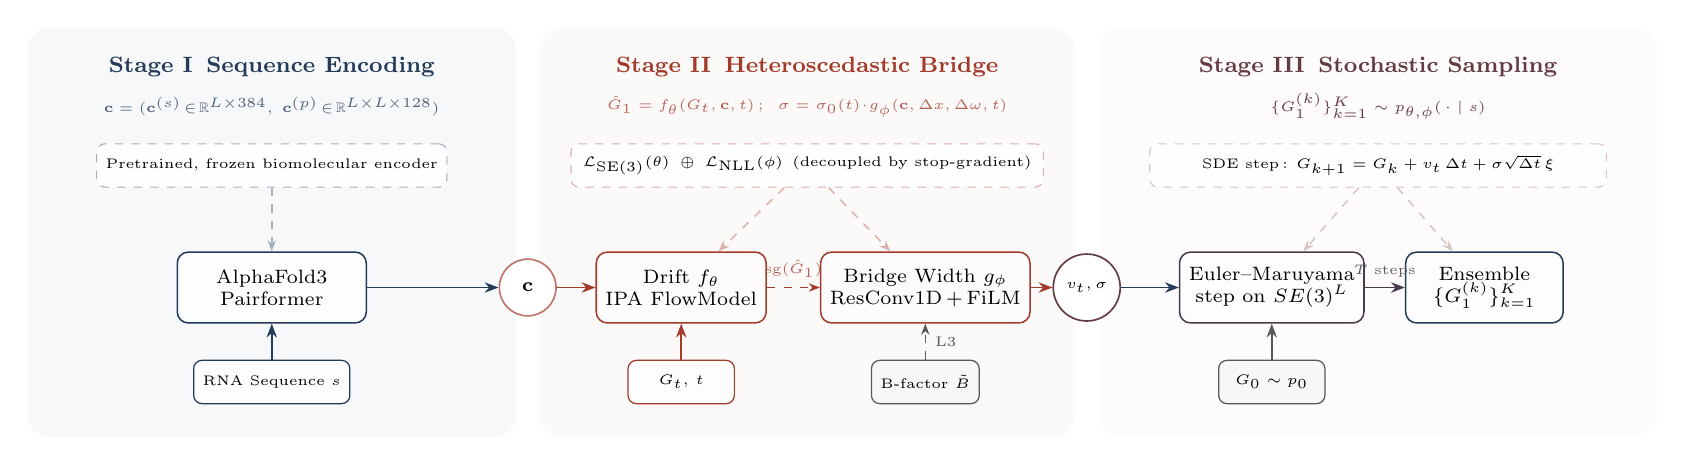
\begin{tikzpicture}[
    module/.style={rounded corners=4pt, minimum height=0.9cm, minimum width=1.8cm,
        align=center, font=\scriptsize, draw, line width=0.55pt, fill=white},
    detail/.style={rounded corners=3pt, minimum height=0.55cm, minimum width=1.8cm,
        align=center, font=\tiny, fill=white, draw=cvneutral!40, line width=0.4pt, dashed},
    ext/.style={rounded corners=3pt, minimum height=0.55cm, minimum width=1.35cm,
        align=center, font=\tiny, fill=white, draw, line width=0.45pt},
    hand/.style={circle, minimum size=0.72cm,
        align=center, font=\scriptsize, draw, line width=0.6pt, fill=white},
    arr/.style={-{Stealth[length=5pt]}, line width=0.65pt},
    darr/.style={-{Stealth[length=4pt]}, line width=0.55pt, dashed},
    lbl/.style={font=\tiny, text=cvneutral},
]

% ===== Stage backgrounds =====
\begin{scope}[on background layer]
  \fill[cvsubtlesoft!35, rounded corners=8pt] (-0.3,-1.9) rectangle (5.9,3.3);
  \fill[cvaccentsoft!30, rounded corners=8pt] (6.2,-1.9) rectangle (13.0,3.3);
  \fill[cvsubtlesoft!18!cvaccentsoft!18, rounded corners=8pt] (13.3,-1.9) rectangle (20.4,3.3);
\end{scope}

% ===== Stage labels with key quantities =====
\node[font=\footnotesize\bfseries, cvsubtle] at (2.8, 2.8)
  {Stage I\enskip Sequence Encoding};
\node[font=\tiny, cvsubtle!80] at (2.8, 2.3)
  {$\mathbf{c}=(\mathbf{c}^{(s)}\!\in\!\mathbb{R}^{L\times 384},\;\mathbf{c}^{(p)}\!\in\!\mathbb{R}^{L\times L\times 128})$};

\node[font=\footnotesize\bfseries, cvaccent] at (9.6, 2.8)
  {Stage II\enskip Heteroscedastic Bridge};
\node[font=\tiny, cvaccent!80] at (9.6, 2.3)
  {$\hat{G}_1=f_\theta(G_t,\mathbf{c},t)\,;\;\;\sigma=\sigma_0(t)\!\cdot\!g_\phi(\mathbf{c},\Delta x,\Delta\omega,t)$};

\node[font=\footnotesize\bfseries, cvsubtle!50!cvaccent] at (16.85, 2.8)
  {Stage III\enskip Stochastic Sampling};
\node[font=\tiny, cvsubtle!50!cvaccent] at (16.85, 2.3)
  {$\{G_1^{(k)}\}_{k=1}^{K}\sim p_{\theta,\phi}(\,\cdot\mid s)$};

% ===== STAGE I: Sequence Encoding =====
\node[detail, draw=cvsubtle!40, fill=cvsubtlesoft!5, minimum width=3.6cm] (l1) at (2.8, 1.55)
  {Pretrained, frozen biomolecular encoder};

\node[module, draw=cvsubtle, fill=cvsubtlesoft!12, minimum width=2.4cm] (af3) at (2.8, 0)
  {AlphaFold3\\Pairformer};

\draw[darr, cvsubtle!40] (l1) -- (af3);

\node[ext, draw=cvsubtle, fill=cvsubtlesoft!8] (seq) at (2.8, -1.2)
  {RNA Sequence $s$};
\draw[arr, cvsubtle] (seq) -- (af3);

% ===== Handoff: c =====
\node[hand, draw=cvaccent!70] (handI) at (6.05, 0) {$\mathbf{c}$};
\draw[arr, cvsubtle] (af3.east) -- (handI.west);

% ===== STAGE II: Heteroscedastic Bridge =====
\node[detail, draw=cvaccent!40, fill=cvaccentsoft!6, minimum width=6.0cm] (l2) at (9.6, 1.55)
  {$\mathcal{L}_{\mathrm{SE(3)}}(\theta)\;\oplus\;\mathcal{L}_{\mathrm{NLL}}(\phi)$\enskip(decoupled by stop-gradient)};

\node[module, draw=cvaccent, fill=cvaccentsoft!18, minimum width=1.9cm] (drift) at (8.0, 0)
  {Drift $f_\theta$\\IPA FlowModel};
\node[module, draw=cvaccent, fill=cvaccentsoft!18, minimum width=2.5cm] (bw) at (11.1, 0)
  {Bridge Width $g_\phi$\\ResConv1D\,+\,FiLM};

\draw[arr, cvaccent] (handI.east) -- (drift.west);
\draw[darr, cvaccent] (drift.east) -- (bw.west)
  node[midway, above, font=\tiny, text=cvaccent!80] {$\mathrm{sg}(\hat{G}_1)$};
\draw[darr, cvaccent!40] (l2) -- (drift);
\draw[darr, cvaccent!40] (l2) -- (bw);

% Inputs
\node[ext, draw=cvaccent, fill=cvaccentsoft!8] (gt) at (8.0, -1.2)
  {$G_t,\,t$};
\node[ext, draw=cvneutral, fill=black!3] (bf) at (11.1, -1.2)
  {B-factor $\tilde{B}$};
\draw[arr, cvaccent] (gt) -- (drift);
\draw[darr, cvneutral] (bf) -- (bw) node[midway, right, lbl] {L3};

% ===== Handoff: (v_t, σ) =====
\node[hand, minimum size=0.85cm, draw=cvaccent!50!cvsubtle, font=\tiny] (handII) at (13.15, 0)
  {$v_t,\sigma$};
\draw[arr, cvaccent] (bw.east) -- (handII.west);

% ===== STAGE III: Stochastic Sampling =====
\node[detail, draw=cvsubtle!30!cvaccent!30, fill=cvsubtlesoft!4!cvaccentsoft!4, minimum width=5.8cm] (l3) at (16.85, 1.55)
  {SDE step\,: $G_{k+1}=G_k+v_t\,\Delta t+\sigma\sqrt{\Delta t}\,\xi$};

\node[module, draw=cvsubtle!70!cvaccent, fill=cvsubtlesoft!8!cvaccentsoft!8, minimum width=2.0cm] (em) at (15.5, 0)
  {Euler--Maruyama\\step on $SE(3)^L$};
\node[module, draw=cvsubtle, fill=cvsubtlesoft!10, minimum width=2.0cm] (ens) at (18.2, 0)
  {Ensemble\\$\{G_1^{(k)}\}_{k=1}^{K}$};

\draw[arr, cvsubtle] (handII.east) -- (em.west);
\draw[arr, cvsubtle!70!cvaccent] (em.east) -- (ens.west)
  node[midway, above, lbl] {$T$ steps};
\draw[darr, cvsubtle!30!cvaccent!30] (l3) -- (em);
\draw[darr, cvsubtle!30!cvaccent!30] (l3) -- (ens);

% Input
\node[ext, draw=cvneutral, fill=black!3] (g0) at (15.5, -1.2)
  {$G_0\sim p_0$};
\draw[arr, cvneutral] (g0) -- (em);

\end{tikzpicture}%
}
\caption{\textbf{ResBridge framework.}
\textbf{Stage~I.} An RNA sequence $s$ is encoded once by a frozen AlphaFold3 Pairformer~\cite{abramson2024af3} into a single representation $\mathbf{c}^{(s)}\!\in\!\mathbb{R}^{L\times 384}$ and a pair representation $\mathbf{c}^{(p)}\!\in\!\mathbb{R}^{L\times L\times 128}$, jointly written $\mathbf{c}$.
\textbf{Stage~II.} The deterministic drift $f_\theta$ of \S\ref{sec:se3-fm} consumes $(G_t,\mathbf{c},t)$ and predicts the clean state $\hat{G}_1$, supervised by the SE(3) regression loss \eqref{eq:fm-loss}. The bridge width network $g_\phi$ reuses the same $\mathbf{c}$ and the geometric residuals \eqref{eq:geom-residual} computed from \emph{stop-gradient} $\hat{G}_1$, and emits per-residue bounded modulations $\alpha^{m}_i\!\in\![\alpha_{\min},\alpha_{\max}]$ that scale the endpoint-safe base schedule into $\sigma^{m}_{i,t}=\sigma_{0}^{m}(t)\!\cdot\!\alpha^{m}_{i}$, trained by the heteroscedastic NLL \eqref{eq:bridge-nll}. The dashed \textsf{sg} arrow is the architectural \emph{stop-gradient firewall} that decouples the two losses: gradients of $\mathcal{L}_{\mathrm{NLL}}$ never reach $\theta$, so $f_\theta$ converges to the same vector field as in the deterministic SE(3) flow matching backbone. The optional B-factor anchor (Level~3, \S\ref{sec:resbridge-guided}) supplies an experimental flexibility prior on $\sigma$.
\textbf{Stage~III.} The drift velocity $v_t$ and the bridge width $\sigma$ enter a single Euler--Maruyama step on $SE(3)^L$ \eqref{eq:bridge-em}; iterating $T$ steps from independent $G_0\!\sim\!p_0$ produces a conformational ensemble $\{G_1^{(k)}\}_{k=1}^{K}$.}
\label{fig:framework}
\end{figure}

The deterministic SE(3) flow matching backbone of \S\ref{sec:se3-fm} learns a velocity field that, given any starting frame configuration $G_0\!\sim\!p_0$, integrates to a single endpoint via an ODE. Under multi-modal data this leaves the model two routes to under-coverage of $p_{\mathrm{data}}(\,\cdot\mid s)$: (i) the velocity field, trained by an $L_2$ regression onto a deterministic conditional path, can be biased toward the conditional mean whenever multiple ground-truth endpoints are consistent with the same $(G_t,s)$; and (ii) the noise-free sampler offers no second mechanism to disperse trajectories across distinct basins once one has been committed to. We address both routes simultaneously by wrapping the deterministic drift with a per-residue heteroscedastic noise process whose width is itself learned from the drift's own residuals, turning the ODE of \S\ref{sec:se3-fm} into an SDE that we call \textbf{ResBridge}.

\paragraph{Stochastic bridge on $SE(3)^L$.}
Let $f_\theta$ denote the drift model trained by \eqref{eq:fm-loss}, and write $\hat{G}_1=(\hat{x}_1,\hat{R}_1)=f_\theta(G_t,s,t)$ for the clean state implied by its prediction at $(G_t,s,t)$, with corresponding velocities $\hat{v}^{x}_{t}=(\hat{x}_{1}-x_{t})/(1{-}t)$ and $\hat{v}^{R}_{t}=\log(R_{t}^{\!\top}\hat{R}_{1})/(1{-}t)$. ResBridge integrates the SDE
\begin{equation}
\mathrm{d}x_{i,t}\;=\;\hat{v}^{x}_{i,t}\,\mathrm{d}t \,+\, \sigma^{x}_{i,t}\,\mathrm{d}W^{x}_{t},
\qquad
\mathrm{d}R_{i,t}\;=\;R_{i,t}\!\cdot\!\bigl(\,\hat{v}^{R}_{i,t}\,\mathrm{d}t \,+\, \sigma^{R}_{i,t}\,\mathrm{d}B^{R}_{t}\,\bigr),
\label{eq:bridge-sde}
\end{equation}
where $W^{x}_{t}$ is a standard 3-dimensional Brownian motion in $\mathbb{R}^3$ and $B^{R}_{t}$ is the right-invariant Brownian motion on $SO(3)$ identified with $\mathbb{R}^3$ via $\mathfrak{so}(3)\cong\mathbb{R}^3$. Discretizing \eqref{eq:bridge-sde} by Euler--Maruyama yields the ResBridge sampling step
\begin{equation}
x_{i,t+\Delta t}\;=\;x_{i,t}+\hat{v}^{x}_{i,t}\,\Delta t \,+\, \sigma^{x}_{i,t}\sqrt{\Delta t}\,\xi_i,
\qquad
R_{i,t+\Delta t}\;=\;R_{i,t}\,\exp\!\bigl(\,\hat{v}^{R}_{i,t}\,\Delta t \,+\, \sigma^{R}_{i,t}\sqrt{\Delta t}\,\zeta_i\,\bigr),
\label{eq:bridge-em}
\end{equation}
with $\xi_i,\zeta_i\!\sim\!\mathcal{N}(0,I_3)$ independent across residues and time steps. The right-hand sides recover the deterministic flow-matching update of \S\ref{sec:se3-fm} exactly when $\sigma^{x}_{i,t}=\sigma^{R}_{i,t}=0$, so ResBridge strictly generalizes its backbone.

We construct the bridge width as a product of two factors,
\begin{equation}
\sigma^{m}_{i,t}\;=\;\sigma_{0}^{m}(t)\cdot\alpha^{m}_{i,t},
\qquad
\sigma_{0}^{m}(t)\;=\;\lambda_m\sqrt{t(1-t)},
\qquad m\in\{x,R\},
\label{eq:bridge-width}
\end{equation}
where $\sigma_{0}^{m}(t)$ is a global \emph{endpoint-safe} base schedule and $\alpha^{m}_{i,t}\in[\alpha_{\min},\alpha_{\max}]$ is a per-residue, state-dependent modulation predicted by an auxiliary network $g_\phi$ described below. Three properties of \eqref{eq:bridge-width} together give ResBridge its expressive power. (i) \emph{Endpoint safety}: $\sigma_{0}^{m}(t)$ vanishes at $t\!=\!0$ and $t\!=\!1$, so the SDE collapses back to deterministic transport at both ends and trajectories are guaranteed to land on the data manifold rather than be perturbed off it by terminal noise. (ii) \emph{Per-residue}: each nucleotide carries its own $\sigma$, so the model can spread a flexible loop without perturbing a stable helix elsewhere in the same molecule. (iii) \emph{State-dependence}: $\alpha^{m}_{i,t}$ depends on the current backbone state $G_t$ \emph{and} on the drift's prediction at that state, so the noise can ramp up exactly where the drift is uncertain along the present trajectory; the bound $[\alpha_{\min},\alpha_{\max}]$ then keeps SDE integration numerically stable throughout training and inference.

The drift in \eqref{eq:bridge-sde} is unchanged from \S\ref{sec:se3-fm}: ResBridge does not retrain the drift, it only learns how much noise to inject around it. Any pretrained SE(3) flow matching backbone can therefore be retrofitted simply by attaching $g_\phi$ and replacing the ODE sampler by \eqref{eq:bridge-em}.

\paragraph{Bridge width network.}
The auxiliary network $g_\phi$ that predicts $\alpha_{i,t}$ --- the \emph{bridge width network} --- takes four kinds of input at every residue $i$: the per-residue context $\mathbf{c}^{(s)}_i$ and the pairwise context $\{\mathbf{c}^{(p)}_{ij}\}_{j=1}^{L}$ already exposed by $f_\theta$ in its forward pass; the geometric residuals
\begin{equation}
\Delta x_{i}\;=\;x_{i,t}-\hat{x}_{i,1},\qquad
\Delta\omega_{i}\;=\;\log\!\bigl(\hat{R}_{i,1}^{\!\top}R_{i,t}\bigr)\in\mathbb{R}^{3},
\label{eq:geom-residual}
\end{equation}
which summarize how far the present state has drifted from $f_\theta$'s clean prediction; and the timestep $t$. The single, geometric, and pair features are linearly projected into a shared hidden representation, fused additively after a mean pool of $\mathbf{c}^{(p)}$ over its second axis, FiLM-conditioned~\cite{perez2018film} on a sinusoidal embedding of $t$, and processed by a stack of residual 1D convolutional blocks; two LayerNorm--linear heads then emit a translational and a rotational pre-activation $u^{x}_i,u^{R}_i$, mapped to bounded modulations by
\begin{equation}
\alpha^{m}_{i}\;=\;\alpha_{\min}+(\alpha_{\max}-\alpha_{\min})\,\mathrm{sigmoid}(u^{m}_i),\qquad m\in\{x,R\}.
\label{eq:alpha-bound}
\end{equation}

Two design choices in the input set are essential. First, the pair representation $\mathbf{c}^{(p)}$ is the only signal that lets $g_\phi$ tell apart structurally distinct conformers of the \emph{same} sequence: a sequence-only network would be forced to predict identical $\sigma$ profiles for every member of an ensemble, whereas pair features encode the ambient structural context that the drift has resolved at the current trajectory point and so vary across modes. Second, the geometric residuals \eqref{eq:geom-residual} are computed from \emph{detached} drift outputs; together with the stop-gradient that we apply to the residuals appearing in the loss below, this is the architectural manifestation of the principle that $g_\phi$ is purely an \emph{observer} of $f_\theta$ and never sends gradients back into the drift parameters $\theta$.

\paragraph{Heteroscedastic self-regulating NLL.}
We train $g_\phi$ by placing a Gaussian predictive model on the magnitude of the drift residual,
\begin{equation}
r^{x}_{i}\;=\;\bigl\|\,\mathrm{sg}(\hat{x}_{i,1})-x_{i,1}\,\bigr\|_{2},\qquad
r^{R}_{i}\;=\;\bigl\|\log\bigl(R_{i,1}^{\!\top}\,\mathrm{sg}(\hat{R}_{i,1})\bigr)\bigr\|_{2},
\label{eq:bridge-residual}
\end{equation}
and minimizing the per-residue heteroscedastic negative log-likelihood
\begin{equation}
\mathcal{L}_{\mathrm{NLL}}(\phi)\;=\;\mathbb{E}_{t,G_0,G_1}\!\left[\,\frac{1}{L}\sum_{i=1}^{L}\,\sum_{m\in\{x,R\}}\lambda_m\!\left(\frac{(r^{m}_{i})^{2}}{(\sigma^{m}_{i,t})^{2}}+\log(\sigma^{m}_{i,t})^{2}\right)\right],
\label{eq:bridge-nll}
\end{equation}
where $\mathrm{sg}(\cdot)$ is the stop-gradient operator, $G_1=(x_{i,1},R_{i,1})_{i=1}^{L}$ is the data sample, the modality weights $\lambda_x,\lambda_R$ are inherited from \eqref{eq:fm-loss} so that $\sigma$ stays in raw physical units (\AA{} for translation, rad for rotation), and the gradient of \eqref{eq:bridge-nll} flows only into $\phi$.

The choice of \eqref{eq:bridge-nll} is what makes the bridge \emph{self-regulating}. Differentiating with respect to $\sigma^{m}_{i,t}$ and setting the result to zero gives the closed-form per-residue minimizer
\begin{equation}
\sigma^{m,\star}_{i,t}\;=\;r^{m}_{i},
\label{eq:bridge-optimal}
\end{equation}
so that the optimal heteroscedastic Gaussian fit assigns each residue a noise standard deviation \emph{equal to the magnitude of its own current drift error}. Two consequences follow that drive the behavior of ResBridge at sampling time. First, on residues where the drift is already accurate ($r^{m}_i$ small), $\sigma^{m}_{i,t}$ is driven down toward zero --- those residues are essentially deterministically transported --- whereas on residues where the drift is uncertain ($r^{m}_i$ large), $\sigma^{m}_{i,t}$ is driven up so that the SDE injects exploratory noise exactly where it is most needed. Second, because $r^{m}_i$ depends on the conformer-specific clean prediction $\hat{G}_1$ and on the pair context $\mathbf{c}^{(p)}$ that distinguishes structural members of the same sequence, the optimum \eqref{eq:bridge-optimal} is itself conformer-specific: a residue that is rigid in one structural family of a given sequence and flexible in another receives different $\sigma$ profiles in the two cases, and the corresponding bridges therefore explore different basins of $p_{\mathrm{data}}(\,\cdot\mid s)$. This is the mechanism by which ResBridge converts a single-mode deterministic flow into a multi-modal ensemble sampler.

\eqref{eq:bridge-nll} also admits a clean Bayesian reading: viewing $f_\theta(G_t,s,t)$ as a frozen point estimate of the unknown clean state $G_1$, $\sigma^{m}_{i,t}$ plays the role of a learned per-residue \emph{posterior standard deviation} of $G_1\mid G_t,s$, calibrated against the empirical residual distribution by the same loss that trains heteroscedastic regression and probabilistic depth networks~\cite{kendall2017uncertainties}. In our setting, however, $\sigma$ is not merely an inference-time uncertainty estimate: it is fed straight back into the SDE \eqref{eq:bridge-sde} as the actual noise injected during sampling, so calibration to the drift residual translates directly into the spread of the generated ensemble.

In implementation, $f_\theta$ and $g_\phi$ share a single forward pass --- $g_\phi$ reuses the $\hat{G}_1$, $\mathbf{c}^{(s)}$, and $\mathbf{c}^{(p)}$ already produced by $f_\theta$ --- but are updated by two separate AdamW optimizers, one for $\theta$ minimizing \eqref{eq:fm-loss} and one for $\phi$ minimizing \eqref{eq:bridge-nll}. The stop-gradient in \eqref{eq:bridge-residual} and the detached residuals in \eqref{eq:geom-residual} together guarantee that the two losses do not interfere: from $\theta$'s perspective the bridge does not exist, so the drift continues to converge to the same vector field as in \S\ref{sec:se3-fm}; from $\phi$'s perspective $\theta$ is a frozen oracle, so calibration of $\sigma$ is a stationary supervised regression problem.

\subsection{ResBridge-guided}\label{sec:resbridge-guided}


\paragraph{B-factor as physical flexibility.}



Papers to be submitted to NeurIPS 2026 must be prepared according to the
instructions presented here. Papers may only be up to {\bf nine} pages long, including figures. \textbf{Papers that exceed the page limit will not be reviewed (or in any other way considered) for presentation at the conference.}
Additional pages \emph{containing acknowledgments, references, checklist, and optional technical appendices} do not count as content pages. 


The margins in 2026 are the same as those in previous years.


Authors are required to use the NeurIPS \LaTeX{} style files obtainable at the NeurIPS website as indicated below. Please make sure you use the current files and not previous versions. Tweaking the style files may be grounds for desk rejection.


\subsection{Retrieval of style files}


The style files for NeurIPS and other conference information are available on the website at
\begin{center}
  \url{https://neurips.cc}.
\end{center}
% The file \verb+neurips_2026.pdf+ contains these instructions and illustrates the various formatting requirements your NeurIPS paper must satisfy.


The only supported style file for NeurIPS 2026 is \verb+neurips_2026.sty+, rewritten for \LaTeXe{}. \textbf{Previous style files for \LaTeX{} 2.09,  Microsoft Word, and RTF are no longer supported.}


The \LaTeX{} style file contains three optional arguments: 
\begin{itemize}
\item \verb+final+, which creates a camera-ready copy, 
\item \verb+preprint+, which creates a preprint for submission to, e.g., arXiv, \item \verb+nonatbib+, which will not load the \verb+natbib+ package for you in case of package clash.
\end{itemize}


\paragraph{Preprint option}
If you wish to post a preprint of your work online, e.g., on arXiv, using the NeurIPS style, please use the \verb+preprint+ option. This will create a nonanonymized version of your work with the text ``Preprint. Work in progress.'' in the footer. This version may be distributed as you see fit, as long as you do not say which conference it was submitted to. Please \textbf{do not} use the \verb+final+ option, which should \textbf{only} be used for papers accepted to NeurIPS.


At submission time, please omit the \verb+final+ and \verb+preprint+ options. This will anonymize your submission and add line numbers to aid review. Please do \emph{not} refer to these line numbers in your paper as they will be removed during generation of camera-ready copies.


The file \verb+neurips_2026.tex+ may be used as a ``shell'' for writing your paper. All you have to do is replace the author, title, abstract, and text of the paper with your own.


The formatting instructions contained in these style files are summarized in Sections \ref{gen_inst}, \ref{headings}, and \ref{others} below.


\section{General formatting instructions}
\label{gen_inst}


The text must be confined within a rectangle 5.5~inches (33~picas) wide and
9~inches (54~picas) long. The left margin is 1.5~inch (9~picas).  Use 10~point
type with a vertical spacing (leading) of 11~points.  Times New Roman is the
preferred typeface throughout, and will be selected for you by default.
Paragraphs are separated by \nicefrac{1}{2}~line space (5.5 points), with no
indentation.


The paper title should be 17~point, initial caps/lower case, bold, centered
between two horizontal rules. The top rule should be 4~points thick and the
bottom rule should be 1~point thick. Allow \nicefrac{1}{4}~inch space above and
below the title to rules. All pages should start at 1~inch (6~picas) from the
top of the page.


For the final version, authors' names are set in boldface, and each name is
centered above the corresponding address. The lead author's name is to be listed
first (left-most), and the co-authors' names (if different address) are set to
follow. If there is only one co-author, list both author and co-author side by
side.


Please pay special attention to the instructions in Section \ref{others}
regarding figures, tables, acknowledgments, and references.

\section{Headings: first level}
\label{headings}


All headings should be lower case (except for first word and proper nouns),
flush left, and bold.


First-level headings should be in 12-point type.


\subsection{Headings: second level}


Second-level headings should be in 10-point type.


\subsubsection{Headings: third level}


Third-level headings should be in 10-point type.


\paragraph{Paragraphs}


There is also a \verb+\paragraph+ command available, which sets the heading in
bold, flush left, and inline with the text, with the heading followed by 1\,em
of space.


\section{Citations, figures, tables, references}
\label{others}


These instructions apply to everyone.


\subsection{Citations within the text}


The \verb+natbib+ package will be loaded for you by default.  Citations may be
author/year or numeric, as long as you maintain internal consistency.  As to the
format of the references themselves, any style is acceptable as long as it is
used consistently.


The documentation for \verb+natbib+ may be found at
\begin{center}
  \url{http://mirrors.ctan.org/macros/latex/contrib/natbib/natnotes.pdf}
\end{center}
Of note is the command \verb+\citet+, which produces citations appropriate for
use in inline text.  For example,
\begin{verbatim}
   \citet{hasselmo} investigated\dots
\end{verbatim}
produces
\begin{quote}
  Hasselmo, et al.\ (1995) investigated\dots
\end{quote}


If you wish to load the \verb+natbib+ package with options, you may add the
following before loading the \verb+neurips_2026+ package:
\begin{verbatim}
   \PassOptionsToPackage{options}{natbib}
\end{verbatim}


If \verb+natbib+ clashes with another package you load, you can add the optional
argument \verb+nonatbib+ when loading the style file:
\begin{verbatim}
   \usepackage[nonatbib]{neurips_2026}
\end{verbatim}


As submission is double blind, refer to your own published work in the third
person. That is, use ``In the previous work of Jones et al.\ [4],'' not ``In our
previous work [4].'' If you cite your other papers that are not widely available
(e.g., a journal paper under review), use anonymous author names in the
citation, e.g., an author of the form ``A.\ Anonymous'' and include a copy of the anonymized paper in the supplementary material.


\subsection{Footnotes}


Footnotes should be used sparingly.  If you do require a footnote, indicate
footnotes with a number\footnote{Sample of the first footnote.} in the
text. Place the footnotes at the bottom of the page on which they appear.
Precede the footnote with a horizontal rule of 2~inches (12~picas).


Note that footnotes are properly typeset \emph{after} punctuation
marks.\footnote{As in this example.}


\subsection{Figures}


\begin{figure}
  \centering
  \fbox{\rule[-.5cm]{0cm}{4cm} \rule[-.5cm]{4cm}{0cm}}
  \caption{Sample figure caption. Explain what the figure shows and add a key take-away message to the caption.}
\end{figure}


All artwork must be neat, clean, and legible. Lines should be dark enough for
 reproduction purposes. The figure number and caption always appear after the
figure. Place one line space before the figure caption and one line space after
the figure. The figure caption should be lower case (except for the first word and proper nouns); figures are numbered consecutively.


You may use color figures.  However, it is best for the figure captions and the
paper body to be legible if the paper is printed in either black/white or in
color.


\subsection{Tables}


All tables must be centered, neat, clean, and legible.  The table number and
title always appear before the table.  See Table~\ref{sample-table}.


Place one line space before the table title, one line space after the
table title, and one line space after the table. The table title must
be lower case (except for the first word and proper nouns); tables are
numbered consecutively.


Note that publication-quality tables \emph{do not contain vertical rules}. We
strongly suggest the use of the \verb+booktabs+ package, which allows for
typesetting high-quality, professional tables:
\begin{center}
  \url{https://www.ctan.org/pkg/booktabs}
\end{center}
This package was used to typeset Table~\ref{sample-table}.


\begin{table}
  \caption{Sample table caption. Explain what the table shows and add a key take-away message to the caption.}
  \label{sample-table}
  \centering
  \begin{tabular}{lll}
    \toprule
    \multicolumn{2}{c}{Part}                   \\
    \cmidrule(r){1-2}
    Name     & Description     & Size ($\mu$m) \\
    \midrule
    Dendrite & Input terminal  & $\approx$100     \\
    Axon     & Output terminal & $\approx$10      \\
    Soma     & Cell body       & up to $10^6$  \\
    \bottomrule
  \end{tabular}
\end{table}

\subsection{Math}
Note that display math in bare TeX commands will not create correct line numbers for submission. Please use LaTeX (or AMSTeX) commands for unnumbered display math. (You really shouldn't be using \$\$ anyway; see \url{https://tex.stackexchange.com/questions/503/why-is-preferable-to} and \url{https://tex.stackexchange.com/questions/40492/what-are-the-differences-between-align-equation-and-displaymath} for more information.)

\subsection{Final instructions}

Do not change any aspects of the formatting parameters in the style files.  In
particular, do not modify the width or length of the rectangle the text should
fit into, and do not change font sizes. Please note that pages should be
numbered.


\section{Preparing PDF files}


Please prepare submission files with paper size ``US Letter,'' and not, for
example, ``A4.''


Fonts were the main cause of problems in the past years. Your PDF file must only
contain Type 1 or Embedded TrueType fonts. Here are a few instructions to
achieve this.


\begin{itemize}


\item You should directly generate PDF files using \verb+pdflatex+.


\item You can check which fonts a PDF files uses.  In Acrobat Reader, select the
  menu Files$>$Document Properties$>$Fonts and select Show All Fonts. You can
  also use the program \verb+pdffonts+ which comes with \verb+xpdf+ and is
  available out-of-the-box on most Linux machines.


\item \verb+xfig+ ``patterned'' shapes are implemented with bitmap fonts.  Use
  "solid" shapes instead.


\item The \verb+\bbold+ package almost always uses bitmap fonts.  You should use
  the equivalent AMS Fonts:
\begin{verbatim}
   \usepackage{amsfonts}
\end{verbatim}
followed by, e.g., \verb+\mathbb{R}+, \verb+\mathbb{N}+, or \verb+\mathbb{C}+
for $\mathbb{R}$, $\mathbb{N}$ or $\mathbb{C}$.  You can also use the following
workaround for reals, natural and complex:
\begin{verbatim}
   \newcommand{\RR}{I\!\!R} %real numbers
   \newcommand{\Nat}{I\!\!N} %natural numbers
   \newcommand{\CC}{I\!\!\!\!C} %complex numbers
\end{verbatim}
Note that \verb+amsfonts+ is automatically loaded by the \verb+amssymb+ package.


\end{itemize}


If your file contains type 3 fonts or non embedded TrueType fonts, we will ask
you to fix it.


\subsection{Margins in \LaTeX{}}


Most of the margin problems come from figures positioned by hand using
\verb+\special+ or other commands. We suggest using the command
\verb+\includegraphics+ from the \verb+graphicx+ package. Always specify the
figure width as a multiple of the line width as in the example below:
\begin{verbatim}
   \usepackage[pdftex]{graphicx} ...
   \includegraphics[width=0.8\linewidth]{myfile.pdf}
\end{verbatim}
See Section 4.4 in the graphics bundle documentation
(\url{http://mirrors.ctan.org/macros/latex/required/graphics/grfguide.pdf})


A number of width problems arise when \LaTeX{} cannot properly hyphenate a
line. Please give LaTeX hyphenation hints using the \verb+\-+ command when
necessary.

\begin{ack}
Use unnumbered first level headings for the acknowledgments. All acknowledgments
go at the end of the paper before the list of references. Moreover, you are required to declare
funding (financial activities supporting the submitted work) and competing interests (related financial activities outside the submitted work).
More information about this disclosure can be found at: \url{https://neurips.cc/Conferences/2026/PaperInformation/FundingDisclosure}.


Do {\bf not} include this section in the anonymized submission, only in the final paper. You can use the \texttt{ack} environment provided in the style file to automatically hide this section in the anonymized submission.
\end{ack}

{
\small
\nocite{alexander1995template,bower1995genesis,hasselmo1995dynamics}
\bibliographystyle{plainnat}
\bibliography{neurips_2026}
}


%%%%%%%%%%%%%%%%%%%%%%%%%%%%%%%%%%%%%%%%%%%%%%%%%%%%%%%%%%%%

\appendix


\section{Pseudocode}

%==============================================================
% Three aligned pseudocode columns: L1 / L2 / L3.
% Single 3-column tabular: shared lines align horizontally and
% lines unique to L2/L3 leave blank cells in the lower levels.
%==============================================================
\begin{figure}[t]
\centering
\setlength{\tabcolsep}{3pt}
\renewcommand{\arraystretch}{1.15}
\newcommand{\addLtwo}[1]{\textcolor{blue!70!black}{#1}}
\newcommand{\addLthree}[1]{\textcolor{red!70!black}{#1}}
\newcommand{\Ln}[1]{\makebox[1.7em][l]{#1.}}
\footnotesize
\begin{tabular}{@{}>{\raggedright\arraybackslash}p{0.32\textwidth} >{\raggedright\arraybackslash}p{0.32\textwidth} >{\raggedright\arraybackslash}p{0.32\textwidth}@{}}
\toprule
\textbf{Algorithm 1.} & \textbf{Algorithm 2.} & \textbf{Algorithm 3.} \\
\textsl{Level~1: SE(3) flow matching} & \textsl{Level~2: ResBridge} & \textsl{Level~3: ResBridge-guided} \\
\midrule
\multicolumn{3}{@{}l}{\textsl{Training}} \\
\Ln{1} Sample $(s,G_1)\!\sim\!\mathcal{D}$, $G_0\!\sim\!p_0$
  & \Ln{1} Sample $(s,G_1)\!\sim\!\mathcal{D}$, $G_0\!\sim\!p_0$
  & \Ln{1} Sample $(s,G_1\addLthree{,B})\!\sim\!\mathcal{D}$, $G_0\!\sim\!p_0$ \\
\Ln{2} $t\!\sim\!U(0,1)$;\; $G_t\!\leftarrow\!\mathrm{interp}(G_0,G_1,t)$
  & \Ln{2} $t\!\sim\!U(0,1)$;\; $G_t\!\leftarrow\!\mathrm{interp}(G_0,G_1,t)$
  & \Ln{2} $t\!\sim\!U(0,1)$;\; $G_t\!\leftarrow\!\mathrm{interp}(G_0,G_1,t)$ \\
\Ln{3} $\hat{G}_1\!\leftarrow\!f_\theta(G_t,s,t)$
  & \Ln{3} $\hat{G}_1\addLtwo{,\,\mathbf{c}}\!\leftarrow\!f_\theta(G_t,s,t)$
  & \Ln{3} $\hat{G}_1\addLtwo{,\,\mathbf{c}}\!\leftarrow\!f_\theta(G_t,s,t)$ \\
\Ln{4} $\mathcal{L}_{\mathrm{drift}}\!\leftarrow\!\|G_1-\hat{G}_1\|^2$
  & \Ln{4} $\mathcal{L}_{\mathrm{drift}}\!\leftarrow\!\|G_1-\hat{G}_1\|^2$
  & \Ln{4} $\mathcal{L}_{\mathrm{drift}}\!\leftarrow\!\|G_1-\hat{G}_1\|^2$ \\
  & \addLtwo{\Ln{5} $r\!\leftarrow\!\mathrm{sg}(\|G_1-\hat{G}_1\|)$}
  & \addLtwo{\Ln{5} $r\!\leftarrow\!\mathrm{sg}(\|G_1-\hat{G}_1\|)$} \\
  & \addLtwo{\Ln{6} $\alpha\!\leftarrow\!g_\phi(\mathbf{c},G_t,\mathrm{sg}(\hat{G}_1),t)$}
  & \addLtwo{\Ln{6} $\alpha\!\leftarrow\!g_\phi(\mathbf{c},G_t,\mathrm{sg}(\hat{G}_1),t)$} \\
  & \addLtwo{\Ln{7} $\sigma\!\leftarrow\!\sigma_0(t)\cdot\alpha$}
  & \addLtwo{\Ln{7} $\sigma\!\leftarrow\!\sigma_0(t)\cdot\alpha$} \\
  & \addLtwo{\Ln{8} $\mathcal{L}_{\mathrm{NLL}}\!\leftarrow\!r^2/\sigma^2+\log\sigma^2$}
  & \addLtwo{\Ln{8} $\mathcal{L}_{\mathrm{NLL}}\!\leftarrow\!r^2/\sigma^2+\log\sigma^2$} \\
  &
  & \addLthree{\Ln{9} $\tilde{B}\!\leftarrow\!\mathrm{norm}_{+}(B)$} \\
  &
  & \addLthree{\Ln{10} $\mathcal{L}_{\mathrm{bf}}\!\leftarrow\!\|\alpha-\tilde{B}\|^2$} \\
\Ln{5} $\theta\!\leftarrow\!\mathrm{Adam}(\nabla_\theta\mathcal{L}_{\mathrm{drift}})$
  & \Ln{9} $\theta\!\leftarrow\!\mathrm{Adam}(\nabla_\theta\mathcal{L}_{\mathrm{drift}})$
  & \Ln{11} $\theta\!\leftarrow\!\mathrm{Adam}(\nabla_\theta\mathcal{L}_{\mathrm{drift}})$ \\
  & \addLtwo{\Ln{10} $\phi\!\leftarrow\!\mathrm{Adam}(\nabla_\phi\mathcal{L}_{\mathrm{NLL}})$}
  & \addLtwo{\Ln{12} $\phi\!\leftarrow\!\mathrm{Adam}(\nabla_\phi(\mathcal{L}_{\mathrm{NLL}}\addLthree{+\lambda_B\mathcal{L}_{\mathrm{bf}}}))$} \\
\addlinespace
\multicolumn{3}{@{}l}{\textsl{Sampling}} \\
\Ln{1} $G_0\!\sim\!p_0$
  & \Ln{1} $G_0\!\sim\!p_0$
  & \Ln{1} $G_0\!\sim\!p_0$ \\
\Ln{2} \textbf{for} $k=0,\ldots,K{-}1$ \textbf{do}
  & \Ln{2} \textbf{for} $k=0,\ldots,K{-}1$ \textbf{do}
  & \Ln{2} \textbf{for} $k=0,\ldots,K{-}1$ \textbf{do} \\
\Ln{3} \quad $t\!\leftarrow\!k/K$
  & \Ln{3} \quad $t\!\leftarrow\!k/K$
  & \Ln{3} \quad $t\!\leftarrow\!k/K$ \\
\Ln{4} \quad $\hat{G}_1\!\leftarrow\!f_\theta(G_t,s,t)$
  & \Ln{4} \quad $\hat{G}_1\addLtwo{,\,\mathbf{c}}\!\leftarrow\!f_\theta(G_t,s,t)$
  & \Ln{4} \quad $\hat{G}_1\addLtwo{,\,\mathbf{c}}\!\leftarrow\!f_\theta(G_t,s,t)$ \\
\Ln{5} \quad $v_t\!\leftarrow\!(\hat{G}_1-G_t)/(1{-}t)$
  & \Ln{5} \quad $v_t\!\leftarrow\!(\hat{G}_1-G_t)/(1{-}t)$
  & \Ln{5} \quad $v_t\!\leftarrow\!(\hat{G}_1-G_t)/(1{-}t)$ \\
  & \addLtwo{\Ln{6} \quad $\alpha\!\leftarrow\!g_\phi(\mathbf{c},G_t,\hat{G}_1,t)$}
  & \addLtwo{\Ln{6} \quad $\alpha\!\leftarrow\!g_\phi(\mathbf{c},G_t,\hat{G}_1,t)$} \\
  & \addLtwo{\Ln{7} \quad $\sigma\!\leftarrow\!\sigma_0(t)\cdot\alpha$;\; $\xi\!\sim\!\mathcal{N}(0,I)$}
  & \addLtwo{\Ln{7} \quad $\sigma\!\leftarrow\!\sigma_0(t)\cdot\alpha$;\; $\xi\!\sim\!\mathcal{N}(0,I)$} \\
\Ln{6} \quad $G_{t+\Delta t}\!\leftarrow\!G_t+v_t\Delta t$
  & \Ln{8} \quad $G_{t+\Delta t}\!\leftarrow\!G_t+v_t\Delta t\,\addLtwo{+\,\sigma\sqrt{\Delta t}\,\xi}$
  & \Ln{8} \quad $G_{t+\Delta t}\!\leftarrow\!G_t+v_t\Delta t\,\addLtwo{+\,\sigma\sqrt{\Delta t}\,\xi}$ \\
\Ln{7} \textbf{return} $G_1$
  & \Ln{9} \textbf{return} $G_1$
  & \Ln{9} \textbf{return} $G_1$ \\
\bottomrule
\end{tabular}
\caption{\textbf{The three levels of ResBridge, aligned row by row.} A single three-line table; each row corresponds to one conceptual operation, so identical lines line up horizontally and a level that does not contain a given operation simply leaves its cell blank. \textcolor{blue!70!black}{Blue} marks every line (or sub-expression) that Level~2 introduces on top of Level~1 (the heteroscedastic stochastic bridge); \textcolor{red!70!black}{red} marks every line (or sub-expression) that Level~3 introduces on top of Level~2 (the B-factor anchor). Both colors persist across columns so that the layering remains visible at a glance. \emph{Notation.} $f_\theta$: drift FlowModel, returning the predicted clean state $\hat{G}_1$ and (in Level~2/3) its single/pair embeddings $\mathbf{c}$; $g_\phi$: BridgeWidthNet, returning a per-residue bounded modulation $\alpha\in[\alpha_{\min},\alpha_{\max}]$; $\sigma_0(t)=\lambda\sqrt{t(1{-}t)}$: endpoint-safe base schedule; $\sigma$: per-residue bridge width; $\mathrm{sg}(\cdot)$: stop-gradient, decoupling drift gradients from $g_\phi$; $\mathrm{norm}_{+}$: log-shift-scale positive normalization of B-factors. The drift parameters $\theta$ and the bridge parameters $\phi$ are updated by \emph{separate} optimizers, which is what keeps the bridge purely an ``observer'' of the drift.}
\label{fig:algorithms}
\end{figure}


\section{Technical appendices and supplementary material}
Technical appendices with additional results, figures, graphs, and proofs may be submitted with the paper submission before the full submission deadline (see above). You can upload a ZIP file for videos or code, but do not upload a separate PDF file for the appendix. There is no page limit for the technical appendices. 

Note: Think of the appendix as ``optional reading'' for reviewers. The paper must be able to stand alone without the appendix; for example, adding critical experiments that support the main claims to an appendix is inappropriate. 

%%%%%%%%%%%%%%%%%%%%%%%%%%%%%%%%%%%%%%%%%%%%%%%%%%%%%%%%%%%%

\newpage
\input{checklist.tex}


\end{document}
